\documentclass[a4paper]{article}
\usepackage[T1]{fontenc}			% \chapter package
\usepackage[english]{babel}
\usepackage[english]{isodate}  		% date format
\usepackage{graphicx}				% manage images
\usepackage{amsfonts}
\usepackage{booktabs}				% high quality tables
\usepackage{amsmath}				% math package
\usepackage{amssymb}				% another math package (e.g. \nexists)
\usepackage{bm}                     % bold math symbols
\usepackage{mathtools}				% emphasize equations
\usepackage{stmaryrd} 				% '\llbracket' and '\rrbracket'
\usepackage{amsthm}					% better theorems
\usepackage{enumitem}				% manage list
\usepackage{pifont}					% nice itemize
\usepackage{cancel}					% cancel math equations
\usepackage{caption}				% custom caption
\usepackage[]{mdframed}				% box text
\usepackage{multirow}				% more lines in a table
\usepackage{textcomp, gensymb}		% degree symbol
\usepackage[x11names]{xcolor}		% RGB color
\usepackage[many]{tcolorbox}		% colorful box
\usepackage{multicol}				% more rows in a table (used for the lists)
\usepackage{listings}
\usepackage{url}
\usepackage{qrcode}
\usepackage{fontawesome5}
\usepackage{ragged2e}
\usepackage{cite}                   % references
\usepackage{imakeidx}               % index
\makeindex[program=makeindex, columns=1,
           title=Index, 
           intoc,
           options={-s index-style.ist}]
\usepackage{fancyhdr}
\usepackage{eurosym}                % Euro symbol package
\usepackage{moreverb}               % verbatim to fix white lines in code snippets (mathescape problem with lstlisting)

%\pdfcompresslevel=0
%\pdfobjcompresslevel=0

\definecolor{codegreen}{rgb}{0,0.6,0}
\definecolor{codegray}{rgb}{0.5,0.5,0.5}
\definecolor{codepurple}{rgb}{0.58,0,0.82}
%\definecolor{backcolour}{rgb}{0.95,0.95,0.92}
\definecolor{backcolour}{rgb}{255,255,255}
\lstdefinestyle{mystyle}{
	backgroundcolor=\color{backcolour},   
	commentstyle=\color{codegreen},
	keywordstyle=\color{magenta},
	numberstyle=\tiny\color{codegray},
	stringstyle=\color{codepurple},
	basicstyle=\ttfamily\footnotesize,
	breakatwhitespace=false,         
	breaklines=true,                 
	captionpos=b,                    
	keepspaces=true,                 
	numbers=left,                    
	numbersep=5pt,                  
	showspaces=false,                
	showstringspaces=false,
	showtabs=false,                  
	tabsize=2,
    mathescape,
    frame=lines
}

\lstdefinelanguage{pseudo-code}{
	keywords={while, do, for, if},
	keywordstyle=\color{Red2}\bfseries,
	ndkeywords={},
	ndkeywordstyle=\color{darkgray}\bfseries,
	identifierstyle=\color{black},
	sensitive=false,
	comment=[l]{//},
	morecomment=[s]{/*}{*/},
	commentstyle=\color{codegreen}\ttfamily,
	stringstyle=\color{red}\ttfamily,
	morestring=[b]',
	morestring=[b]"
}

\lstset{
	language=pseudo-code,
	backgroundcolor=\color{lightgray},
	extendedchars=true,
	basicstyle=\footnotesize\ttfamily,
	showstringspaces=false,
	showspaces=false,
	numbers=left,
	numberstyle=\footnotesize,
	numbersep=9pt,
	tabsize=2,
	breaklines=true,
	showtabs=false,
	captionpos=b
}

\lstset{style=mystyle}


% thanks Mico: https://tex.stackexchange.com/a/60218/312896
\makeatletter
\renewcommand\paragraph{\@startsection{paragraph}{4}{\z@}%
            {-2.5ex\@plus -1ex \@minus -.25ex}%
            {1.25ex \@plus .25ex}%
            {\normalfont\normalsize\bfseries}}
\makeatother
\setcounter{secnumdepth}{4} % how many sectioning levels to assign numbers to
\setcounter{tocdepth}{4}    % how many sectioning levels to show in ToC


% draw a frame around given text
\newcommand{\framedtext}[1]{%
	\par%
	\noindent\fbox{%
		\parbox{\dimexpr\linewidth-2\fboxsep-2\fboxrule}{#1}%
	}%
}


% table of content links
\usepackage{xcolor}
\usepackage[linkcolor=black, citecolor=blue, urlcolor=cyan]{hyperref} % hypertexnames=false
\hypersetup{
	colorlinks=true
}


\newtheorem{theorem}{\textcolor{Red3}{\underline{Theorem}}}
\renewcommand{\qedsymbol}{QED}
\newcommand{\dquotes}[1]{``#1''}
\newcommand{\longline}{\noindent\rule{\textwidth}{0.4pt}}
\newcommand{\circledtext}[1]{\raisebox{.5pt}{\textcircled{\raisebox{-.9pt}{#1}}}}
\newcommand{\definition}[1]{\textcolor{Red3}{\textbf{#1}}\index{#1}}
\newcommand{\definitionWithSpecificIndex}[2]{\textcolor{Red3}{\textbf{#1}}\index{#2}}
\newcommand{\example}[1]{\textcolor{Green4}{\textbf{#1}}}
\newcommand{\highspace}{\vspace{1.2em}\noindent}
\newcommand{\opt}{\mathrm{opt} \:}
\renewcommand{\lstlistingname}{Algorithm}
\renewcommand{\lstlistlistingname}{Algorithms}
\newcommand{\version}{v0.3.1-dev}


\begin{document}
    \newcounter{definition}[section]
    \newcounter{example}[section]
    \newcounter{exercise}[section]
    
    \newtcolorbox[use counter = definition]{definitionbox}[1][]{%
        breakable,
        enhanced,
        colback=red!5!white,
        colframe=red!75!black,
        fonttitle=\bfseries,
        title={Definition \thetcbcounter#1} %
    }

    \newtcolorbox[use counter = exercise]{exercisebox}[1][]{%
        breakable,
        enhanced,
        colback=Red3!5!white,
        colframe=Red3!75!black,
        fonttitle=\bfseries,
        title={Exercise \thetcbcounter#1} %
    }
    
    \newtcolorbox[use counter = example]{examplebox}[1][]{%
        breakable,
        enhanced,
        colback=Green4!5!white,
        colframe=Green4!75!black,
        fonttitle=\bfseries,
        title={Example \thetcbcounter#1} %
    }

    \newtcolorbox[]{deepeningbox}[1][]{%
        breakable,
        enhanced,
        colback=DarkOrange3!5!white,
        colframe=DarkOrange3!75!black,
        fonttitle=\bfseries,
        title={Deepening#1} %
    }

    %%%%%%%%%%%%%%%
    % Notes cover %
    %%%%%%%%%%%%%%%
    \author{260236}
\title{Parallel Computing - Notes - \version}
\date{\printdayoff\today}
\maketitle

    %%%%%%%%%%%
    % Preface %
    %%%%%%%%%%%
	\section*{Preface}

Every theory section in these notes has been taken from the sources:
\begin{itemize}
    \item Course slides.\cite{numerical-linear-algebra-polimi}
\end{itemize}
About:
\begin{itemize}
    \item[\faIcon{github}] \href{https://github.com/PoliMI-HPC-E-notes-projects-AndreVale69/HPC-E-PoliMI-university-notes}{GitHub repository}
    \begin{center}
        \qrcode{https://github.com/PoliMI-HPC-E-notes-projects-AndreVale69/HPC-E-PoliMI-university-notes}
    \end{center}
\end{itemize}
These notes are an unofficial resource and shouldn't replace the course material or any other book on numerical linear algebra. It is not made for commercial purposes. I've made the following notes to help me improve my knowledge and maybe it can be helpful for everyone.

As I have highlighted, a student should choose the teacher's material or a book on the topic. These notes can only be a helpful material.

\highspace

\subsection*{Correlated Projects}

During the Numerical Linear Algebra for HPC course, I was part of a team where we created a project that included two challenges related to the course. See more details in the corresponding repository:
\begin{itemize}
    \item[\faIcon{github}] \href{https://github.com/PoliMI-HPC-E-notes-projects-AndreVale69/NLA-challenges}{GitHub repository}
    \begin{center}
        \qrcode{https://github.com/PoliMI-HPC-E-notes-projects-AndreVale69/NLA-challenges}
    \end{center}
\end{itemize}

    %%%%%%%%%%%%%%%%%%%%%
    % Table of contents %
    %%%%%%%%%%%%%%%%%%%%%
    \tableofcontents
    \newpage

    %%%%%%%%%%%%
    % Listings %
    %%%%%%%%%%%%
    \lstlistoflistings

    %%%%%%%%%%%%%%%%
    % Introduction %
    %%%%%%%%%%%%%%%%
    \section{Introduction}

\begin{definitionbox}
    \definition{Operations Research (OR)}, often shortened to the initialism \texttt{OR}, is the branch of mathematics in which \textbf{mathematical models} and \textbf{quantitative methods} (e.g. optimization, game theory, simulation) are \textbf{used to analyze complex decision-making problems} and \textbf{find (near-)optimal solutions}.
\end{definitionbox}

\highspace
The overall and primary \emph{goal} is to \emph{help make better decisions}.

\highspace
OR can be seen as an interdisciplinary field at the intersection of applied mathematics, computer science, economics, and industrial engineering.

\highspace
Operations research is often concerned with \textbf{determining the extreme values of some real-world objective}: the \emph{maximum} (of profit, performance, or yield) or \emph{minimum} (of loss, risk, or cost). Originating in military efforts before World War II, its techniques have grown to concern problems in a variety of industries.\cite{wikipediaOperationsResearch}

\longline

\subsection{Decision-making problems}

Decision-making problems are analyzed using mathematical models and quantitative methods.

\begin{definitionbox}
    \definition{Decision-making problems} are problems in which we must \textbf{choose} a (feasible) \textbf{solution among a large number of alternatives based on one or several criteria}.
\end{definitionbox}

\highspace
Some practical \example{examples} include network design, shortest paths, staff scheduling, and service management.

\highspace
In other words, they are complex decision-making problems that are \textbf{addressed through a mathematical modeling approach} (mathematical models, algorithms, and computer implementations).
    \subsection{Scheme of an OR study}

The most important and common \textbf{steps} in operational research are:
\begin{enumerate}
    \item \textbf{Problem}. Define the problem;
    \item \textbf{Model}. Build the model;
    \item \textbf{Algorithm}. Select or develop an appropriate algorithm;
    \item \textbf{Implementation}. Implementing or using an efficient computer program;
    \item \textbf{Results}. Analyze the results.
\end{enumerate}

\begin{definitionbox}
    A mathematical \definition{model} is a \textbf{simplified representation of a real-world problem}.
\end{definitionbox}

\noindent
To define a mathematical model, it is necessary to identify the fundamental elements of the problem and the main relationships between them. But \textbf{how can we decide} the \emph{number of decision makers}, the \emph{number of objectives} and the \emph{level of uncertainty in the parameters}? It depends on the environment. If we have:
\begin{itemize}
    \item One decision maker, one object, then we will use \textbf{mathematical programming}.
    \item One decision maker, multiple objectives, then we will use \textbf{multi-objective programming}.
    \item Uncertainty greater than zero, then we will use \textbf{stochastic programming}.
    \item Multiple decision makers, then we will use \textbf{game theory}.
\end{itemize}

\highspace
\begin{examplebox}[: production planning]
    A company produces 3 types of electronic devices: $D_{1}$, $D_{2}$, $D_{3}$; going through 3 main phases of the production process: assembly, refinement and quality control.

    Time (in minutes) required for each phase and product:

    \begin{center}
        \begin{tabular}{@{} c | c c c @{}}
            & $D_{1}$ & $D_{2}$ & $D_{3}$ \\
            \midrule
            Assembly        & $80$ & $70$ & $120$ \\
            Refinement      & $70$ & $90$ & $20$ \\
            Quality control & $40$ & $30$ & $20$
        \end{tabular}
    \end{center}

    Available resources within the planning horizon (depend on the workforce) in minutes:
    \begin{center}
        \begin{tabular}{@{} c | c | c @{}}
            Assembly & Refinement & Quality control \\
            \midrule
            $30'000$ & $25'000$ & $18'000$
        \end{tabular}
    \end{center}

    Unitary profit (in KEuro):
    \begin{center}
        \begin{tabular}{@{} c | c | c @{}}
            $D_{1}$ & $D_{2}$ & $D_{3}$ \\
            \midrule
            $1.6$ & $1$ & $2$
        \end{tabular}
    \end{center}
    
    Assumption: the company can sell whatever it produces.

    \emph{Give a mathematical model for determining a production plan which maximizes the total profit.}

    \begin{itemize}
        \item \textbf{Decision variables}, $x_{j}$ is equal to the number of devices $D_{j}$ produced, for $j = 1, 2, 3$.
        
        \item \textbf{Objective function}: $\max \: z = 1.6x_{1} + 1x_{2} + 2x_{3}$.

        \item \textbf{Constraints}: the production capacity limit for each phase:
        \begin{equation*}
            \begin{array}{rcl}
                80x_{1} + 70x_{2} + 120x_{3} &\le& 30'000 \hspace{2em} \text{(assembly)} \\ [.5em]
                70x_{1} + 90x_{2} + 20x_{3} &\le& 25'000 \hspace{2em} \text{(refinement)} \\ [.5em]
                40x_{1} + 30x_{2} + 20x_{3} &\le& 18'000 \hspace{2em} \text{(quality control)}
            \end{array}
        \end{equation*}

        \item \textbf{Non-negative variables}: $x_{1}, x_{2}, x_{3} \ge 0$ may be fractional (real) values.
    \end{itemize}
\end{examplebox}

\begin{examplebox}[: portfolio selection problem]
    An insurance company must decide which investments to select out of a given set of possible assets (stocks, bonds, options, gold certificates, real estate, \dots).

    \begin{center}
        \begin{tabular}{@{} c | c c c @{}}
            Investments & area & capital $\left(c_{j} \: K€\right)$ & expected return $\left(r_{j}\right)$ \\
            \midrule
            A & Germany & $150$ & $11\%$ \\
            B & Italy & $150$ & $9\%$ \\
            C & U.S.A. & $60$ & $13\%$ \\
            D & Italy & $100$ & $10\%$ \\
            E & Italy & $125$ & $8\%$ \\
            F & France & $100$ & $7\%$ \\
            G & Italy & $50$ & $3\%$ \\
            H & UK & $80$ & $5\%$
        \end{tabular}
    \end{center}
    Legend:
    \begin{itemize}
        \item A and B: automotive
        \item C and D: ICT
        \item E and F: real estate
        \item G: short term treasury bounds
        \item H: long term treasury bounds
    \end{itemize}
    The available capital is: $600$ KEuro.

    At most 5 investments to avoid excessive fragmentation.

    Geographic diversification to limit risk: $\le 3$ investments in Italy and $\le 3$ abroad.

    \emph{Give a mathematical model for deciding which investments to select so as to maximize the expected return while satisfying the constraints.}

    \begin{itemize}
        \item \textbf{Decision variables}, $x_{j}$ is equal to $1$ if $j$-th investment is selected and $x_{j}=0$ otherwise, for $j = 1, \dots, 8$.
        
        \item \textbf{Objective function}: $\max \: z = \displaystyle\sum_{j=1}^{8} c_{j} \: r_{j} \: x_{j}$.

        \item \textbf{Constraints}:
        \begin{equation*}
            \begin{array}{rclcl}
                \displaystyle\sum_{j=1}^{8}c_{j} \: x_{j} &\le& 600 &\hspace{1em}& \text{(capital)} \\ [2em]
                \displaystyle\sum_{j=1}^{8}x_{j} &\le& 5 &\hspace{1em}& \text{(max 5 investments)} \\ [2em]
                x_{2}+x_{4}+x_{5}+x_{7} &\le& 3 &\hspace{1em}& \text{(max 3 in Italy)} \\ [.5em]
                x_{1}+x_{3}+x_{6}+x_{8} &\le& 3 &\hspace{1em}& \text{(max 3 abroad)}
            \end{array}
        \end{equation*}

        \item \textbf{Binary (integer) variables}: $x_{j} \in \left\{0,1\right\}$ and $1 \le j \le 8$.
    \end{itemize}

    \underline{\textbf{Possible variant}}. In order to limit the risk, if any of the ICT investment is selected then at least one of the treasury bond must be selected.
    \begin{itemize}
        \item \textbf{Objective function}: $\max z = \displaystyle\sum_{j=1}^{8} c_{j} \: r_{j} \: x_{j}$.

        \item \textbf{Constraints}:
        \begin{equation*}
            \begin{array}{rcll}
                \displaystyle\sum_{j=1}^{8}c_{j} \: x_{j} &\le& 600 & \text{(capital)} \\ [2em]
                \displaystyle\sum_{j=1}^{8}x_{j} &\le& 5 & \text{(max 5 investments)} \\ [2em]
                x_{2}+x_{4}+x_{5}+x_{7} &\le& 3 & \text{(max 3 in Italy)} \\ [.5em]
                x_{1}+x_{3}+x_{6}+x_{8} &\le& 3 & \text{(max 3 abroad)} \\ [1em]
                \dfrac{x_{3} + x_{4}}{2} &\le& x_{7} + x_{8} & \text{(investment in treasury bonds)}
            \end{array}
        \end{equation*}

        \item \textbf{Binary (integer) variables}: $x_{j} \in \left\{0,1\right\}$ and $1 \le j \le 8$.
    \end{itemize}
\end{examplebox}

\newpage

\begin{examplebox}[: facility location]
    Consider 3 oil pits, located in positions $A$, $B$ and $C$, from which oil is extracted.

    \begin{center}
        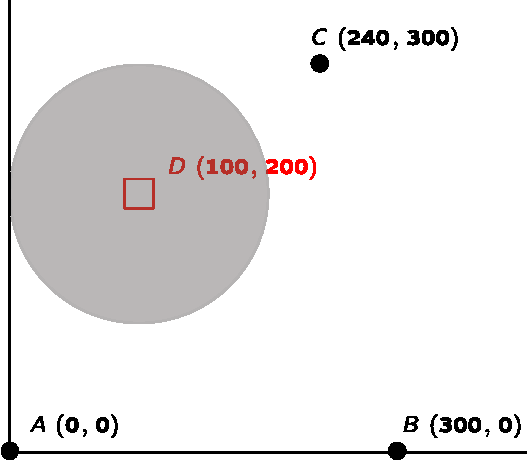
\includegraphics[width=.6\textwidth]{img/facility-location-1.pdf}
    \end{center}

    Connect them to a refinery with pipelines whose cost is proportional to the square of their length.

    The refinery must be at least 100 km away from point $D = \left(100, 200\right)$, but the oil pipelines can cross the corresponding forbidden zone.

    \emph{Give a mathematical model to decide where to locate the refinery so as to minimize the total pipeline cost.}

    \begin{itemize}
        \item \textbf{Decision variables}, $x_{1}, x_{2}$ cartesian coordinates of the refinery.
        
        \item \textbf{Objective function}:
        \begin{equation*}
            \begin{array}{rl}
                \min z = & \left[\left(x_{1} - 0\right)^{2} + \left(x_{2} - 0\right)^{2}\right] + \\ [.5em]
                         & \left[\left(x_{1} - 300\right)^{2} + \left(x_{2} - 0\right)^{2}\right] + \\ [.5em]
                         & \left[\left(x_{1} - 240\right)^{2} + \left(x_{2} - 300\right)^{2}\right]
            \end{array}
        \end{equation*}

        \item \textbf{Constraints}:
        \begin{equation*}
            \sqrt{
                \left(x_{1}-100\right)^{2} + \left(x_{2} - 200\right)^{2}
            } \ge 100
        \end{equation*}

        \item \textbf{Variables}: $x_{1}, x_{2} \in \mathbb{R}$.
    \end{itemize}
\end{examplebox}
    \subsection{Mathematical programming/optimization}

\definition{Mathematical Optimization} or \definition{Mathematical Programming} is the \textbf{selection of a best element}, with regard to some criteria, \textbf{from some set of available alternatives}.

In the more general approach, an optimization problem consists of \textbf{maximizing} or \textbf{minimizing a real function} by systematically choosing input values from within an allowed set and computing the value of the function. The generalization of optimization theory and techniques to other formulations constitutes a large area of applied mathematics.

\highspace
\begin{flushleft}
    \textcolor{Green3}{\faIcon{question-circle} \textbf{And where should we start?}}
\end{flushleft}
Decision-making problems are characterized by a \textbf{single decision maker}, a \textbf{single objective}, and \textbf{reliable parameter estimates}. Using mathematical language, we can say:
\begin{equation*}
    \opt f\left(\mathbf{x}\right) \hspace{1em} \text{with} \hspace{1em} \mathbf{x} \in X \hspace{1em} \text{and} \hspace{1em} \opt = \begin{Bmatrix}
        \min \\ \max
    \end{Bmatrix}
\end{equation*}
Where:
\begin{itemize}
    \item $\mathbf{x} \in \mathbb{R}^{n}$ \textbf{decision variables}. They are numerical variables whose values identify a solution of the problem.

    \item $X \subseteq \mathbb{R}^{n}$ \textbf{feasible region}. Distinguishes between feasible and infeasible solutions (via constraints):
    \begin{equation*}
        X = \left\{\mathbf{x} \in \mathbb{R}^{n} \: : \: g_{i}\left(\mathbf{x}\right) \begin{Bmatrix}
        = \\ \le \\ \ge
        \end{Bmatrix} 0, i = 1, \dots, m\right\}
    \end{equation*}

    \item $f: X \rightarrow \mathbb{R}$ \textbf{objective function}.Expresses in quantitative terms the value or cost of each feasible solution.
\end{itemize}
Note an interesting observation:
\begin{equation*}
    \max\left\{f\left(\mathbf{x}\right): \: \mathbf{x} \in X\right\} = -\min\left\{-f\left(\mathbf{x}\right): \: \mathbf{x} \in X\right\}
\end{equation*} 
    \subsection{Multi-objective programming}\label{subsection: Multi-objective programming}

\begin{flushleft}
    \textcolor{Green3}{\faIcon{question-circle} \textbf{How is it born?}}
\end{flushleft}
Even though some real-word problems can be reduced to a matter of a single objective very often it is hard to define all the aspects in terms of a single objective. Defining multiple objectives often gives a better idea of the task.

\highspace
\definition{Multi-objective programming} (also known as \definition{Multi-objective optimization} or \definition{Pareto optimization}) is an \textbf{area of multiple-criteria decision making} that is concerned with mathematical optimization problems involving \textbf{more than one objective function to be optimized simultaneously}. Multi-objective is a type of vector optimization that has been applied in many fields of science, including engineering, economics and logistics where optimal decisions need to be taken in the presence of trade-offs between two or more conflicting objectives. 

Minimizing cost while maximizing comfort while buying a car, and maximizing performance whilst minimizing fuel consumption and emission of pollutants of a vehicle are \example{examples} of multi-objective optimization problems involving two and three objectives, respectively.\cite{abraham2005evolutionary}

\highspace
Suppose to minimize $f_{1}\left(\mathbf{x}\right)$ and maximize $f_{2}\left(\mathbf{x}\right)$ (e.g. laptop: $f_{1}$ is cost and $f_{2}\left(\mathbf{x}\right)$ is performance):
\begin{enumerate}
    \item Turn it into a \definition{single objective problem} by expressing the two objectives in terms of the same unit (e.g. monetary unit):
    \begin{equation*}
        \min \lambda_{1}f_{1}\left(\mathbf{x}\right) - \lambda_{2}f_{2}\left(\mathbf{x}\right)
    \end{equation*}
    for appropriate scalars $\lambda_{1}$ and $\lambda_{2}$.

    \item Optimize the \definition{primary objective} function and turn the other objective into a constraint:
    \begin{equation*}
        \underset{x \in \tilde{X}}{\max} f_{2}\left(\mathbf{x}\right) \hspace{1em} \text{where} \hspace{1em} \tilde{X} = \left\{\mathbf{x} \in X \: : \: f_{1}\left(\mathbf{x}\right) \le \varepsilon \right\}
    \end{equation*}
    for appropriate constant $\varepsilon$.
\end{enumerate}
This is a simple introduction, the more detailed explanation will be explained in the following pages.
    \subsection{Mathematical Programming or Simulation?}

Mathematical Programming and Simulation involves \textbf{building a model} and \textbf{designing an algorithm}. And the main differences are:
\begin{table}[!htp]
    \centering
    \begin{tabular}{@{} p{15em} | p{15em} @{}}
        \toprule
        \textbf{Mathematical Programming} & \textbf{Simulation} \\
        \midrule
        Problem can be \dquotes{well} formalized. & Problem is difficult to formalize. \\
        \cmidrule{1-2}
        Algorithm yields a(n optimal) solution. & Algorithm simulates the evolution of the real system and allows to evaluate the performance of alternative solutions. \\
        \cmidrule{1-2}
        The results are \dquotes{certain} & The results need to be interpreted. \\
        \cmidrule{1-2}
        Example: assignment. & Example: service counters. \\
        \bottomrule
    \end{tabular}
    \caption{Major differences between Mathematical Programming and Simulation.}
\end{table}

    %%%%%%%%%%%%%%%%%%%%%%%%%%%%%%%%%%
    % Graph and network optimization %
    %%%%%%%%%%%%%%%%%%%%%%%%%%%%%%%%%%
    \section{Graph and network optimization}

\subsection{Graphs}

\subsubsection{Definitions and characteristics}

In the following section we will explain some basic concepts about the graphs. The terms used are important, and we will use the definition box to highlight these words.

\highspace
\begin{definitionbox}[: graph]
    A \definitionWithSpecificIndex{graph}{Graph} is a pair $G = \left(N,E\right)$, with $N$ a set of \textbf{nodes} or \textbf{vertices} and $E \subseteq N \times N$ a set of \textbf{edges} or \textbf{arcs} connecting them pairwise.
\end{definitionbox}

\highspace
\begin{definitionbox}[: edge]
    An \definitionWithSpecificIndex{edge}{Edge} connecting the nodes $i$ and $j$ is represented by
    \begin{itemize}
        \item Graph undirected: $\left\{i,j\right\}$
        \item Graph directed: $\left(i,j\right)$
    \end{itemize}
\end{definitionbox}

\highspace
\begin{examplebox}
    For \example{example}, a road network which connects $n$ cities can be modelled, by a graph where a city corresponds to a node, and a connection corresponds to an edge.

    \begin{center}
        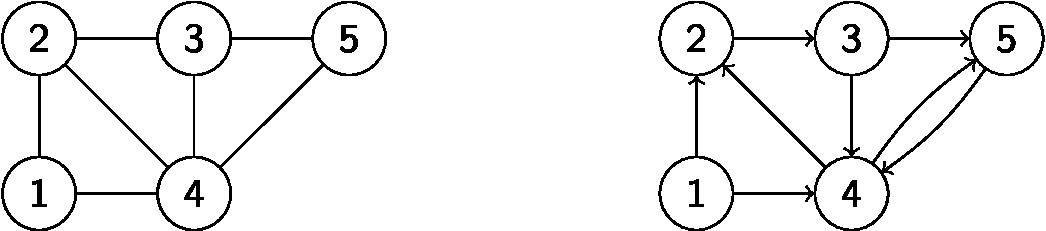
\includegraphics[width=.8\textwidth]{img/graphs-1.pdf}
    \end{center}

    \noindent
    \begin{itemize}
        \item Undirected graph:
        \begin{itemize}
            \item $N = \left\{1,2,3,4,5\right\}$
            \item $E = \left\{
                \left\{1,2\right\},
                \left\{1,4\right\},
                \left\{2,3\right\},
                \left\{2,4\right\},
                \left\{3,4\right\},
                \left\{3,5\right\},
                \left\{4,5\right\}
            \right\}$
        \end{itemize}
        
        \item Directed graph:
        \begin{itemize}
            \item $N = \left\{1,2,3,4,5\right\}$
            \item $E' = \left\{
                \left(1,2\right),
                \left(1,4\right),
                \left(2,3\right),
                \left(2,4\right),
                \left(3,4\right),
                \left(3,5\right),
                \left(4,5\right)
            \right\}$
        \end{itemize}
    \end{itemize}
\end{examplebox}

\newpage

\noindent
Some graph properties are:
\begin{itemize}
    \item Two \textbf{nodes} are \definitionWithSpecificIndex{adjacent}{Adjacent nodes} if they are \textbf{connected by an edge}.

    \item An \textbf{edge} $e$ is \definitionWithSpecificIndex{incident}{Incident edge} in a node $v$ if $v$ is an endpoint of $e$.
    
    In other words, in a graph $G$, two edges are incident \textbf{if they share a common vertex}. For example, edge $E_{1}=\left(v_{1}, v_{2}\right)$ and edge $\left(v_{1}, v_{3}\right)$ are incident as they share the same vertex $v_{1}$.

    \item The degree concept depends on the type of graph:
    \begin{itemize}
        \item Undirected graph: the \definitionWithSpecificIndex{degree}{Node degree} of a node is the \textbf{number of incident edges}.

        \item Directed graph: the \definitionWithSpecificIndex{in-degree}{Node in-degree} and \definitionWithSpecificIndex{out-degree}{Node out-degree} of a node is the \textbf{number of arcs that have it as succesor} and \textbf{predecessor}.
    \end{itemize}
\end{itemize}

\highspace
\begin{examplebox}[: adjacent, incident, degree, in-degree and out-degree]
    Given the graphs:
    
    \begin{center}
        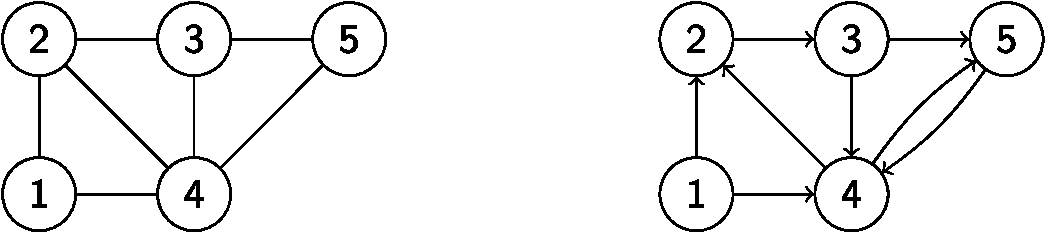
\includegraphics[width=.8\textwidth]{img/graphs-2.pdf}
    \end{center}

    \begin{itemize}
        \item Undirected graph:
        \begin{itemize}
            \item Nodes 1 and 2 are \textbf{adjacent} (unlike nodes 1 and 3).
            \item Edge $\left\{1,2\right\}$ is \textbf{incident} in nodes 1 and 2.
            \item Node 1 has \textbf{degree} 2, node 4 has \textbf{degree} 4.
        \end{itemize}

        \item Directed graph: node 1 has \textbf{in-degree} 0, and \textbf{out-degree} 2.
    \end{itemize}
\end{examplebox}

\highspace
Other useful features include:
\begin{itemize}
    \item A \definitionWithSpecificIndex{(directed) path from $i \in N$ to $j \in N$}{Directed path from $i \in N$ to $j \in N$} is a sequence of (arcs) edges:
    \begin{equation*}
        p = \left\langle \left\{v_{1}, v_{2}\right\}, \left\{v_{2}, v_{3}\right\}, \dots, \left\{v_{k-1}, v_{k}\right\} \right\rangle
    \end{equation*}
    Connecting nodes $v_{1}$ and $v_{k}$, with $\left\{v_{i}, v_{i+1}\right\} \in E$, for $i = 0, \dots, k-1$.

    \item A generic \textbf{node} $u$ and $v$ are \definitionWithSpecificIndex{connected}{Connected nodes} if there is a path connecting them.
    
    \item A \textbf{graph} $\left(N,E\right)$ is \definitionWithSpecificIndex{connected}{Connected graph} if two generic nodes $u,v$ are connected, $\forall u,v \in N$. Recall that in generic graph notation, the variable $N$ represents a set of nodes or vertices and $E$ represents a set of edges or arcs connecting them in pairs.
    
    \item A \textbf{graph} $\left(N,E\right)$ is \definitionWithSpecificIndex{strongly connected}{Strongly connected graph} if two generic nodes $u,v$ are connected by a directed path, $\forall u,v \in N$ (for any node in the set of nodes or vertices of the graph).
\end{itemize}

\highspace
\begin{examplebox}[: directed path, connected nodes, connected graph, strongly connected]
    Given the graphs:
    
    \begin{center}
        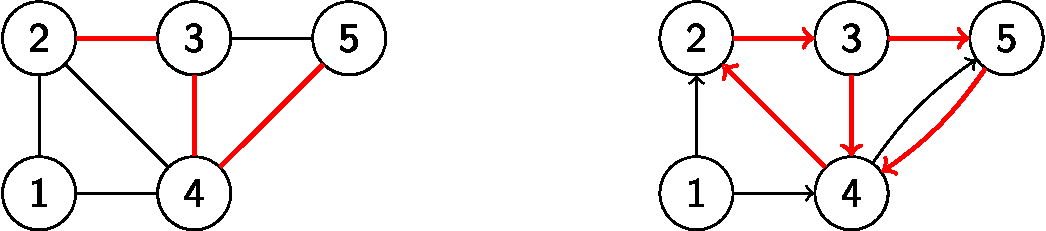
\includegraphics[width=.8\textwidth]{img/graphs-3.pdf}
    \end{center}

    \begin{itemize}
        \item Undirected graph:
        \begin{itemize}
            \item $\left\langle \left\{2,3\right\}, \left\{3,4\right\}, \left\{4,5\right\} \right\rangle$ is a \textbf{path} from node 2 to node 5.
            \item \textbf{Nodes} 2 and 5 are \textbf{connected}.
            \item It is a \textbf{connected graph}.
        \end{itemize}

        \item Directed graph:
        \begin{itemize}
            \item $\left\langle \left\{3,5\right\}, \left\{5,4\right\}, \left\{4,2\right\}, \left\{2,3\right\}, \left\{3,4\right\} \right\rangle$ is a \textbf{directed path} from node 3 to node 4.
            
            \item It is not a \textbf{strongly connected graph} because the node 1 cannot be the destination of none path. In other words, doesn't exist a directed path from node $u$ to node $1$ (where $u$ is a generic node, $\forall u \in N \setminus \left\{1\right\}$).
        \end{itemize}
    \end{itemize}
\end{examplebox}

\highspace
Finally, there are other interesting properties and notations about graphs and edges:
\begin{itemize}
    \item A \definitionWithSpecificIndex{cycle (circuit)}{Cycle in graph}\index{Circuit in graph} is a directed path with $v_{1} = v_{k}$ (source and destination are the same).

    \item A \textbf{graph} is \definitionWithSpecificIndex{bipartite}{Bipartite graph} if there is a partition $N = N_{1} \cup N_{2}$ $\left(N_{1} \cap N_{2} = \emptyset\right)$ such that no edge connects nodes in the same subset.

    \item A \textbf{graph} is \definitionWithSpecificIndex{complete}{Complete graph} if $E = \left\{\left\{v_{j}, v_{j}\right\} \: : \: v_{i}, v_{j} \in N \: \land \: i \le j\right\}$.

    \item Given a directed graph $G = \left(N,A\right)$ and $S \subset N$, the \definitionWithSpecificIndex{outgoing cut}{Outgoing cut} induced by $S$ is:
    \begin{equation*}
        \delta^{+}\left(S\right) = \left\{\left(u,v\right) \in A \: : \: u \in S \: \land : v \in N \subseteq S\right\}
    \end{equation*}
    The \definitionWithSpecificIndex{incoming cut}{Incoming cut} induced by $S$ is:
    \begin{equation*}
        \delta^{-}\left(S\right) = \left\{\left(u,v\right) \in A \: : \: v \in S \: \land : u \in N \subseteq S\right\}
    \end{equation*}
\end{itemize}

\newpage

\begin{examplebox}[: cycle/circuit in graph, bipartite graph, complete graph, out/incoming cut]
    An example of cycle in graph:
    
    \begin{center}
        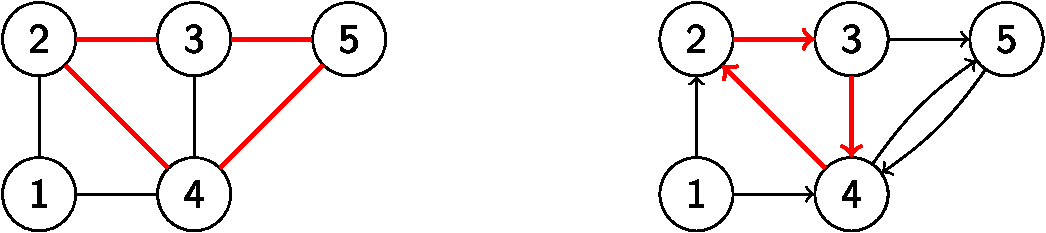
\includegraphics[width=.8\textwidth]{img/graphs-4.pdf}
    \end{center}

    \begin{itemize}
        \item Undirected graph: $\left\langle \left\{2,3\right\}, \left\{3,5\right\}, \left\{5,4\right\}, \left\{4,2\right\} \right\rangle$ is a cycle.
        \item Directed graph: $\left\langle \left(2,3\right), \left(3,4\right), \left(4,2\right) \right\rangle$ is a circuit.
    \end{itemize}
    %
    %

    An example of bipartite/complete graph:

    \begin{center}
        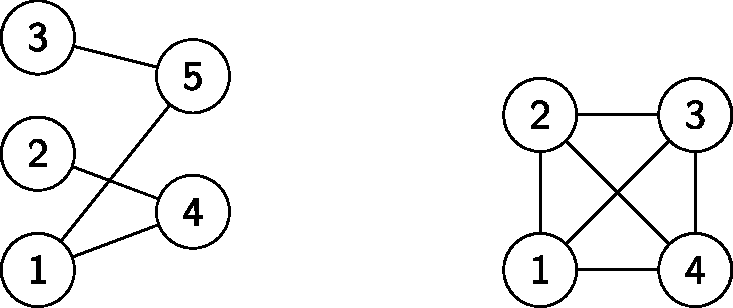
\includegraphics[width=.6\textwidth]{img/graphs-5.pdf}
    \end{center}

    \begin{itemize}
        \item To the left a \textbf{bipartite graph}, because:
        \begin{equation*}
            N_{1} = \left\{1,2,3\right\} \hspace{2em} N_{2} = \left\{4,5\right\}
        \end{equation*}
        \item And to the right a \textbf{complete graph}.
    \end{itemize}
    %
    %

    Finally, an example of out/incoming cut:
    
    \begin{center}
        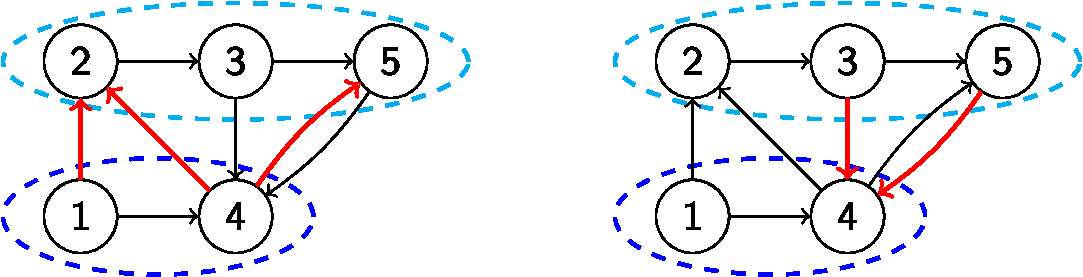
\includegraphics[width=.8\textwidth]{img/graphs-6.pdf}
    \end{center}

    \begin{itemize}
        \item Left graph: 
        \begin{equation*}
            \begin{array}{rcl}
                \delta^{+}\left(\left\{1,4\right\}\right) &=& \left(\left\{1,2\right\}, \left\{4,2\right\}, \left\{4,5\right\}\right) \\ [.5em]
                S &=& \left\{1,4\right\} \\ [.5em]
                N \setminus S &=& \left\{2,3,5\right\}
            \end{array}
        \end{equation*}

        \item Right graph: 
        \begin{equation*}
            \begin{array}{rcl}
                \delta^{-}\left(\left\{1,4\right\}\right) &=& \left(\left\{3,4\right\}, \left\{5,4\right\}\right) \\ [.5em]
                S &=& \left\{1,4\right\} \\ [.5em]
                N \setminus S &=& \left\{2,3,5\right\}
            \end{array}
        \end{equation*}
    \end{itemize}
\end{examplebox}

\subsubsection{Graphical representation}

Such a matrix can easily be represented as a graph. This guarantees that it can be stored efficiently in a computer. But to understand how to do this in general, it's important to understand some other important properties:
\begin{itemize}
    \item For any graph $G$ with $n$ nodes, the \textbf{number of edges} satisfies:
    \begin{itemize}
        \item $m \le \dfrac{n\left(n-1\right)}{2}$ if $G$ is undirected.
        \item $m \le n\left(n-1\right)$ if $G$ is directed.
    \end{itemize}

    \item A graph is \definitionWithSpecificIndex{dense}{Dense graph} if $m \approx n^{2}$ and \definitionWithSpecificIndex{sparse}{Sparse graph} if $m \ll n^{2}$. Where $m$ is the number of arcs and $n$ the number of nodes.

    \item For dense directed graphs, exist an \textbf{adjacency matrix} $A_{n \times n}$:
    \begin{equation*}
        \begin{cases}
            a_{ij} = 1 & \text{if } \left(i,j\right) \in A \\
            a_{ij} = 0 & \text{otherwise}
        \end{cases}
    \end{equation*}
\end{itemize}
To build the adjacency matrix it is necessary to create a \textbf{list of successors} for each node. In other words, for \textbf{each node} we need to write the \textbf{outgoing edges} and write the matrix.
\begin{equation*}
    A = \begin{bmatrix}
        0 & 1 & 0 & 1 & 0 \\
        0 & 0 & 1 & 0 & 0 \\
        0 & 0 & 0 & 1 & 1 \\
        0 & 1 & 0 & 0 & 1 \\
        0 & 0 & 0 & 1 & 0
    \end{bmatrix}
    \hspace{2em}
    \begin{array}{rcl}
        S\left(1\right) &=& \left\{2,4\right\} \\
        S\left(2\right) &=& \left\{3\right\} \\
        S\left(3\right) &=& \left\{4,5\right\} \\
        S\left(4\right) &=& \left\{2,5\right\} \\
        S\left(5\right) &=& \left\{4\right\}
    \end{array}
\end{equation*}
Each row represents a node, and we set the value 1 if the column index is a node that has the arc of the row node as its incoming edge. So row one (node one) has the value one in column two (node two) and column four (node four).

\longline

\subsubsection{Graph reachability problem}

In general the \definitionWithSpecificIndex{graph reachability problem}{Graph reachability problem} can be formulated as follows.

\begin{definitionbox}[: graph reachability problem]
    Given a directed graph $G = \left(N,A\right)$ and a node $s$, determine all the node that are reachable from $s$.
\end{definitionbox}

\noindent
Where $N$ is the set of nodes and $A$ is the set of edges.

\highspace
The problem takes:
\begin{itemize}
    \item As \textbf{input} a \emph{\textbf{graph}} $G = \left(N,A\right)$ described by the successor lists and node $s \in N$.
    
    \item As \textbf{output} produces a \emph{\textbf{subset}} $M \subseteq N$ \emph{\textbf{of nodes}} of the graph $G$ reachable from $s$.
\end{itemize}
Our goal is to devise an efficient algorithm that allows us to find all nodes reachable from $s$.

\newpage

\paragraph{Description and algorithm}

\begin{definitionbox}[: Breadth-First Search]
    \definition{Breadth-First Search (BFS)} is an \textbf{algorithm for searching a tree data structure for a node that satisfies a given property}. It starts at the tree root and explores all nodes at the present depth prior to moving on to the nodes at the next depth level. Extra memory, usually a queue, is needed to keep track of the child nodes that were encountered but not yet explored.
\end{definitionbox}

\begin{lstlisting}[language=pseudo-code, caption={Graph reachability problem: Breadth-First Search}]
Q $\leftarrow$ $\{$s$\}$; $\label{bfs: q-definition}$
M $\leftarrow$ $\emptyset$; $\label{bfs: m-definition}$
while Q $\ne$ $\emptyset$ do: $\label{bfs: while cycle}$
    u $\leftarrow$ node in Q; $\label{bfs: take an element from the queue}$
    Q $\leftarrow$ Q $\setminus$ $\{$u$\}$; $\label{bfs: remove the popped item from the queue}$
    // label u
    M $\leftarrow$ M $\cup$ $\{$u$\}$ $\label{bfs: labeled as explored}$
    for (u, v) $\in$ $\delta^{+}$ (u) do: $\label{bfs: for each tuple in outgoing cut}$
        if v $\notin$ M and v $\notin$ Q: $\label{bfs: if adjacent node is not in reachable set and not in the queue}$
            Q $\leftarrow$ Q $\cup$ $\{$v$\}$ $\label{bfs: add the node v to the queue}$
\end{lstlisting}

\begin{itemize}
    \item[Rows \ref{bfs: q-definition}-\ref{bfs: m-definition}.] Declare a queue \texttt{Q} containing the nodes reachable from the source \texttt{s} and \textbf{not yet processed}. It is managed as a FIFO (First-In First-Out) queue. By definition, we add the \texttt{s} node at the beginning because it is our entry point.
    
    Then we declare the set \texttt{M}. It represents the subset of nodes of the graph that are reachable from the source \texttt{s}. Obviously, it is empty at the beginning of the algorithm.

    \item[Row \ref{bfs: while cycle}.] The BFS algorithm continues to process the nodes until the queue is empty. As long as there is an element, it continues.
    
    \item[Rows \ref{bfs: take an element from the queue}-\ref{bfs: remove the popped item from the queue}.] Take a node from the queue \texttt{Q} and assign it to the variable \texttt{u}. Also remove the element \texttt{u} from the set \texttt{Q}. In other words, perform a difference operation between the sets \texttt{Q} and the set composed only of the element \texttt{u} ($\texttt{Q} \setminus \left\{\texttt{u}\right\}$).
    
    For example, in Python we can get the same result using the \href{https://docs.python.org/3/library/collections.html#collections.deque.popleft}{\texttt{popleft}} method of the \href{https://docs.python.org/3/tutorial/datastructures.html#using-lists-as-queues}{\texttt{deque} data structure}.

    \item[Row \ref{bfs: labeled as explored}.] Using the union between sets, add the visited node \texttt{u} to the subset \texttt{M} of reachable nodes. This operation is also called \dquotes{labeling} because you are \emph{labeling} a node as \emph{visited}.
    
    \item[Row \ref{bfs: for each tuple in outgoing cut}.] Iterate each tuple (node \texttt{u} just popped from the queue, node \texttt{v} adjacent to node \texttt{u}) in the outgoing cut set of node \texttt{u}.
    
    \item[Rows \ref{bfs: if adjacent node is not in reachable set and not in the queue}-\ref{bfs: add the node v to the queue}.] If the adjacent node \texttt{v} is not in the reachable set \texttt{M} and it is not in the queue (so it is not waiting to be evaluated), add the adjacent node \texttt{v} to \texttt{Q} using the union set operation.
\end{itemize}
As we said, the algorithm continues until the queue is not empty. Note that the queue is updated each time a neighboring node is found that is not already in the solution set (\texttt{M}).

\newpage

\paragraph{Complexity of algorithm}

\begin{flushleft}
    \textcolor{Green3}{\faIcon{clock} \textbf{BFS Algorithm - Time Complexity}}
\end{flushleft}
The BFS time complexity%
\footnote{In theoretical computer science, the time complexity is the computational complexity that describes the amount of computer time it takes to run an algorithm. Time complexity is commonly estimated by counting the number of elementary operations performed by the algorithm, supposing that each elementary operation takes a fixed amount of time to perform. Thus, the amount of time taken and the number of elementary operations performed by the algorithm are taken to be related by a constant factor. (\href{https://en.wikipedia.org/wiki/Time_complexity}{source})}
can be expressed as $O\left(\left|N\right|+\left|A\right|\right)$, since \textbf{every node and every edge will be explored in the \underline{worst case}}.
\begin{itemize}
    \item $\left|N\right|$ is the number of \textbf{nodes};
    \item $\left|A\right|$ is the number of \textbf{edges} in the graph.
\end{itemize}
Note that $O\left(\left|A\right|\right)$ may vary between $O\left(1\right)$ and $O\left(N^{2}\right)$, depending on how sparse the input graph is. For example, for \textbf{dense graphs}, exactly $O\left(N^{2}\right)$.

\highspace
\begin{flushleft}
    \textcolor{Green3}{\faIcon{memory} \textbf{BFS Algorithm - Space Complexity}}
\end{flushleft}
When the number of nodes (or vertices) in the graph is known ahead of time, and additional data structures are used to determine which vertices have already been added to the queue, the space complexity%
\footnote{The space complexity of an algorithm or a data structure is the amount of memory space required to solve an instance of the computational problem as a function of characteristics of the input. It is the memory required by an algorithm until it executes completely. This includes the memory space used by its inputs, called input space, and any other (auxiliary) memory it uses during execution, which is called auxiliary space. (\href{https://en.wikipedia.org/wiki/Space_complexity}{source})}
can be expressed as $O\left(\left|N\right|\right)$, where $\left|N\right|$ is the number of vertices. This is in addition to the space required for the graph itself, which may vary depending on the graph representation used by an implementation of the algorithm.

\highspace
In other words, the algorithm needs:
\begin{itemize}
    \item The \textbf{space to store} the set $N$, i.e. the \textbf{set of all nodes} in the graph.
    \item The \textbf{space to store the graph itself} depends on the implementation used.
\end{itemize}

    %%%%%%%%%%%%%%%%%%%
    % Fancy pagestyle %
    %%%%%%%%%%%%%%%%%%%
    \pagestyle{fancy}
    \fancyhead{} % clear all header fields
    \fancyhead[R]{\nouppercase{\leftmark\hfill\rightmark}}

    %%%%%%%%%%%%%%%%%%%%%%%%%%
    % Bibliography and index %
    %%%%%%%%%%%%%%%%%%%%%%%%%%
    \pagestyle{fancy}
\fancyhead{} % clear all header fields
\fancyhead[R]{\nouppercase{\leftmark}}

\bibliography{bibtex}{}
\bibliographystyle{plain}

\newpage

\printindex
\end{document}